\documentclass[../proyecto.tex]{book}

\begin{document}

\chapter{Introducción}

El autómata celular fue inventado por von Neumann y Ulam en 1950 para estudiar el problema de hacer máquinas artificiales que se reproduzcan a sí mismas \cite{neummanUlam}. Con el fin de imitar el comportamiento de seres vivos, el diseño de dichas máquinas incluiría al espacio en el que se desarrollan representado por una malla en la que los nodos son llamados células y evolucionan simultáneamente de acuerdo a un conjunto de reglas simples. Éstas dirigen la "física" de su pequeño universo abstracto. Las reglas son locales en el sentido de que cada célula son "tiene" conocimiento de aquellas células a corta distancia, su vecindario. En la construcción de Neumman el vecindario lo constituyen las células adyacentes verticales y horizontales, lo que se conoce como vecindario de Neumman o de tipo Neumman, si además se considera que las células adyacentes diagonales forman parte del vecindario, entonces pasa a nombrarse vecindario de Moore o de tipo Moore.

El juego de vida es un autómata celular propuesto por Conway en 1970 y popularizado por Martin Gardner en el mismo año \cite{primerap}. Éste consiste en la evolución de una configuración inicial de células con dos estados mutuamente excluyentes, vida (1) o muerte (0), en una malla rectangular infinita dos dimensional. Dicha evolución viene dada por un conjunto de reglas que se aplican simultáneamente a todas las células considerando su vecindario de tipo Moore. Dada una célula viva, ésta continua viviendo si en su vecindario hay 2 o 3 células, en otro caso muere y dada una célula muerta, nace si tiene 3 células en su vecindario.

La elección de las reglas de evolución parecería a priori aleatoria, sin embargo, Conway perseguía con ellas obtener el siguiente comportamiento \cite{libroGardner}:
\begin{itemize}
	\item No debe de haber una configuración inicial de reglas para las cuales haya una prueba simple de que la población pueda crecer sin límite.
	\item Debe de haber configuraciones iniciales que aparentemente crezcan sin límite. 
	\item Debe de haber configuraciones iniciales simples que crezcan y cambien durante un periodo considerable, llegando a tres posibles finales: desaparecer completamente ya sea debido a superpoblación o dispersión, estabilizarse en una configuración que se mantenga constante o entrar en un ciclo sin fin de oscilación de periodo mayor a uno.  
\end{itemize}

Uno de los motivos por los que atrajo la atención de científicos de diferentes campos es la capacidad de observar como patrones complejos surgen de la aplicación de un conjunto muy simple y reducido de reglas. De esta manera comenzaron a observarse configuraciones iniciales que daban lugar a comportamientos interesantes. Tales como las de 'naves espaciales' que se desplazan sobre la malla rectangular, los 'osciladores' que retornan a su configuración inicial después de un número finito de generaciones o las 'vidas inmóviles', osciladores de periodo la unidad.

% Mostrar aquí una imagen con los diferentes estados del oscilador, el bloque y la nave espacial en el tiempo, creo que t=3 es suficiente
\begin{figure}[H]
	\centering
	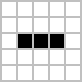
\includegraphics[height=.15\linewidth]{./images/blinker.png}
	\caption{Oscilador de periodo dos nombrado 'Blinker'}
	\label{fig:blinker}
\end{figure} 
\begin{figure}[H]
	
	\centering
	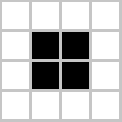
\includegraphics[height=.15\linewidth]{./images/block.png}
	\caption{Vida inmóvil nombrada 'Block'}
	\label{fig:block}
\end{figure} 

Ante la necesidad de realizar simulaciones en los incipientes ordenadores y se enfrentan al problema de representar una malla infinita en un ordenador con memoria finita. Para ello se propone alterar las características topológicas de la malla, imitando las de una botella de Klein, una esfera, o un toro. En particular, esta última resulta atraer gran interés, pues se obtiene evidencia de que reduce los efectos asociados a la finitud de la malla \cite{finitudMalla, finitudMalla2}. Cabe descatar el estudio de la alteración de las cualidades geométricas de la malla, tales como el uso de figuras geométricas regulares diferentes al cuadrado (triángulo y hexágono)\cite{triangular}, teselaciones de Penrose \cite{penrose} o el empleo del espacio geométrico hiperbólico \cite{hiperbolico}. Finalmente, cabe notar que existen implementaciones en las cuales no se almacena la malla en la memoria, si no que se almacena la posición de cada célula respecto a un origen de coordenadas, simulando más eficazmente una malla infinita \cite{boardless}.

El juego de vida también muestra interesantes características en el campo de teoría de la computación. Pertenece a la clase IV de Wolfram \cite{ccuatro, ccuatro2} y se ha demostrado que es una máquina de Turing universal \cite{turingUniversal}. Por tanto existe una configuración inicial que simula una máquina de Turing, la cual fue extendida a una máquina universal de Turing \cite{turing}. Más recientemente en un esfuerzo colectivo, se ha implementado un ordenador con su propio lenguaje ensamblado, compilador a lenguaje de alto nivel, y sobre este último se ha implementado el conocido juego Tetris \cite{tetris, logical}.

Si los autómatas celulares son un modelo que representa a organismos vivos se podría pensar que la hipótesis de actualización simultánea es cuestionable. La existencia de un agente que simultáneamente aplica las reglas a todos los individuos puede hacer que el modelo se aleje demasiado de la realidad que representa. Aunque hay algunos casos en los cuales el comportamiento del autómata celular permanece constante aunque se cambie la hipótesis anterior. En esencia, estamos observando la robustez del modelo a perturbaciones de su evolución. Un modelo será robusto, si pequeños cambios en su evolución se traducirán en pequeñas perturbaciones del comportamiento global del sistema, mientras que si esta pequeña modificación produce un cambio cualitativo en la dinámica del sistema será poco robusto o simplemente sensible a las variaciones en su evolución, dicho cambio cualitativo se conoce también como transición de fase. En la literatura se plantean dos maneras diferentes de introducir la asincronicidad en la aplicación reglas de evolución \cite{asyncIntro}:
\begin{itemize}
	\item \textbf{Evolución totalmente asíncrona}: en cada unidad de tiempo discreto, las reglas de evolución se aplican solamente a un individuo escogido aleatoriamente del conjunto de células.
	\item \textbf{Evolución $\alpha$-asíncrona}: en cada unidad de tiempo discreto, cada células tiene probabilidad $\alpha$ de aplicar las reglas de evolución y probabilidad $1-\alpha$ de mantener su estado.
\end{itemize}

Estos esquemas de evolución también se conocen como \textbf{evolución guiada por pasos} y \textbf{evolución guiada por tiempo}, respectivamente \cite{aka}. Los primeros en estudiar los efectos de la evolución asíncrona frente a la evolución síncrona en el juego de vida fueron \cite{syncVSasync}. Aplicaron un esquema de evolución $\alpha$-asíncrona para mostrar la existencia de una transición de fase de un comportamiento 'estático', donde el sistema termina alcanzando algún punto fijo, a un comportamiento 'vívido'. Posteriormente es estudió como afectaban las variaciones en la topología de la malla a la transición de fase, concluyendo que el valor crítico de la transición de fase depende fuertemente de la regularidad de la malla \cite{mallaIrregular1, mallaIrregular2}.

Hasta donde podemos saber solo se ha estudiado el comportamiento en situaciones de $\alpha$-asincronicidad de configuraciones iniciales aleatorias que rellenan una malla finita, obteniendo resultados que se comparan con las características conocidas del juego de vida síncrono. En este trabajo queremos caracterizar la manera en la que configuraciones iniciales bien conocidas y estudiadas como las que se muestran en las figuras \ref{fig:blinker} y \ref{fig:block}, alteran su comportamiento en situaciones de $\alpha$-asincronicidad, a través de diferentes variables, tales como el número de clústeres de células diferentes por unidad discreta de tiempo, su velocidad y densidad, entre otras.

\end{document}

% !TeX root = ../proyecto.tex
